\subsection{Off-diagonal response certificates}
\label{ssec:r42off}

Condition (FC) concerns forces at different coarse links. Their diagonal
variances need not be small: Proposition~\ref{prop:bpfibreduce}(iv)
identifies their cancellation against the direct same-link curvature.
It is therefore useful to retain the exclusion of the same-link block
throughout a response calculation. The full-row estimate of
Proposition~\ref{prop:integrated-response} remains a valid sufficient
condition; the following statements address the smaller quantity used
by (FC).

\paragraph{The Gaussian restriction on a stronger target.}
Use the Gaussian fibre, precision matrix, marks and heat-bath convention
of Sec.~\ref{round26:sec:ym-relaxation}. Denote its precision parameter by
$\beta_{\rm G}>0$ in this subsection. There are $N_0=L^4$ marks of one
chosen orientation. Let $F_a$ be their centred forces and define
\begin{align}
 C_{ab}&=\Cov(F_a,F_b),\nonumber\\
 X_{ab}&=\int_0^\infty\Cov(F_a,\mathscr P_tF_b)\,dt.
 \label{eq:r42cx}
\end{align}
The matrix $X$ uses the algorithmic heat-bath time, with unit update
rate per free link.\footnote{Multiplying the generator by $c>0$ divides
$X$ by $c$ and leaves $C$ unchanged. That change of clock is not a
construction of a physical transfer Hamiltonian or a physical mass.}

\begin{proposition}\label{prop:r42obstruction}
For this Gaussian family,
\begin{align}
 \|C\|_{\rm op}&\ge6\beta_{\rm G},\nonumber\\
 \|X\|_{\rm op}&\ge
       6\beta_{\rm G}\frac{b^3-1}{b}.\label{eq:r42responsegrowth}
\end{align}
For every metric on the force labels and every $\eta\ge0$,
\begin{equation}\label{eq:r42fullrow}
 \max_a\sum_b e^{\eta d(a,b)}|C_{ab}|\ge6\beta_{\rm G}.
\end{equation}
If $M>0$ is a prescribed parameter metric and
$M^{1/2}XM^{1/2}\le cI$, then, for
$u=N_0^{-1/2}\mathbf1$,
\begin{equation}\label{eq:r42metricnecessary}
 c\ge\frac{6\beta_{\rm G}(b^3-1)}{b\,u^{\mathsf T}M^{-1}u}.
\end{equation}
\end{proposition}
\begin{proof}
The collective-source identities established in
Sec.~\ref{round26:sec:ym-relaxation} give
\begin{align*}
 \mathbf1^{\mathsf T}C\mathbf1&=6\beta_{\rm G}N_0,\\
 \mathbf1^{\mathsf T}X\mathbf1&\ge
              6\beta_{\rm G}N_0(b^3-1)/b.
\end{align*}
Both matrices are nonnegative: the first is a covariance matrix and
the second is the integral of positive spectral correlation matrices.
Evaluate their quadratic forms at the unit vector $u$ to obtain
\eqref{eq:r42responsegrowth}. If $S$ is the maximum unweighted
absolute row sum, then
$6\beta_{\rm G}N_0\le\sum_{a,b}|C_{ab}|\le N_0S$.
Nonnegative exponential weights only increase the sum. Finally the
metric hypothesis is equivalent by congruence to $X\le cM^{-1}$.
Evaluate this inequality at $u$ and use the lower response bound.
\end{proof}

Thus vanishing of a full row, or boundedness of the unscaled response
matrix, is not an attainable Gaussian substitute for (FC) when
$\beta_{\rm G}$ is bounded below and $b$ grows. This restriction is on
the stated Gaussian model and normalization; transferring it to a
different Wilson claim would require a comparison theorem. The metric
in \eqref{eq:r42metricnecessary} must be the metric required by the
downstream estimate, rather than a normalization chosen after the
response has been computed.

\begin{figure}[tb]
\centering
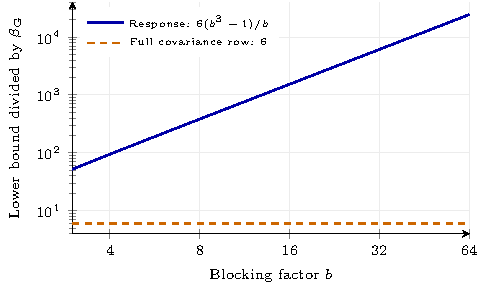
\includegraphics[width=\columnwidth]{figures/r42-gaussian-obstruction.pdf}
\caption{Exact Gaussian lower bounds from
Proposition~\ref{prop:r42obstruction}, divided by $\beta_{\rm G}$.
The curve is $6(b^3-1)/b$ and the horizontal line is $6$. These are
analytic bounds for response and full covariance rows, respectively;
they are not measurements of a physical mass.}
\label{fig:r42growth}
\end{figure}

\begin{figure}[tb]
\centering
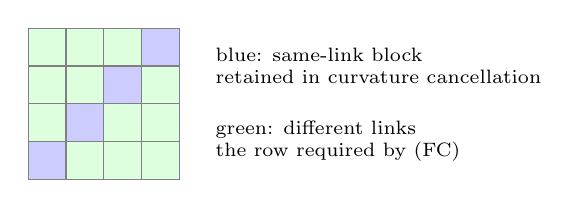
\begin{tikzpicture}[scale=.48,font=\scriptsize]
\foreach \i in {0,...,3}{\foreach \j in {0,...,3}{
 \ifnum\i=\j
  \fill[blue!20] (\i,\j) rectangle +(1,1);
 \else
  \fill[green!13] (\i,\j) rectangle +(1,1);
 \fi
 \draw[gray] (\i,\j) rectangle +(1,1);
}}
\node[align=left,anchor=west] at (4.7,3) {blue: same-link block\\retained in curvature cancellation};
\node[align=left,anchor=west] at (4.7,1) {green: different links\\the row required by (FC)};
\end{tikzpicture}
\caption{The exclusion applies to an entire same-link Lie-algebra block,
not just the diagonal entries in a chosen component basis. Large
self-variances do not prevent small off-diagonal rows.}
\label{fig:r42off}
\end{figure}

\paragraph{A criterion preserving the excluded block.}
Let $P_i$ be finitely many conditional expectations on one real
$L^2(\nu)$ space, and write
\[
 Q_i=I-P_i,\qquad \mathscr L=\sum_iQ_i,\qquad
 \mathscr P_t=e^{-t\mathscr L}.
\]
Let $F_a$ be a finite family of centred $L^2$ observables. Associate each
index $a$ with a coarse link $e(a)$, and give the links a metric $d$.
The indices may include Lie-algebra components. Put $a\sim c$ when
$e(a)=e(c)$. For $\eta\ge0$ set
\begin{align}
 S_\eta^{\ne}&=\sup_a\sum_{c\not\sim a}
   e^{\eta d(e(a),e(c))}|\Cov(F_a,F_c)|,\label{eq:r42soff}\\
 \Theta_\eta(t)&=\sup_a\sum_{c\not\sim a}
   e^{\eta d(e(a),e(c))}
   \sum_i\|Q_iF_a\|_2\|Q_i\mathscr P_tF_c\|_2.
   \label{eq:r42theta}
\end{align}

\begin{proposition}\label{prop:r42semigroup}
Suppose $\ker\mathscr L$ consists of constants. Then
\begin{equation}\label{eq:r42integrated}
 S_\eta^{\ne}\le\int_0^\infty\Theta_\eta(t)\,dt,
\end{equation}
with an infinite right side permitted. No positive uniform spectral
gap is assumed.
\end{proposition}
\begin{proof}
The operator $\mathscr L$ is bounded, self-adjoint and nonnegative.
For finite $T$, differentiation of the bounded exponential gives
\begin{align}
 \Cov(F_a,F_c)
 &=\int_0^T\sum_i
       \langle Q_iF_a,Q_i\mathscr P_tF_c\rangle\,dt\nonumber\\
 &\quad+\langle F_a,\mathscr P_TF_c\rangle.
 \label{eq:r42finiteT}
\end{align}
Here $Q_i^2=Q_i=Q_i^*$ was used. By the spectral theorem,
$\mathscr P_TF_c\to0$ in $L^2$ for every centred $F_c$.
Apply Cauchy--Schwarz to the integrands, sum only over
$c\not\sim a$ with the displayed weights, and take the supremum.
The family is finite, so the absolute remainder row tends to zero.
Let $T\to\infty$. If the integral diverges the inequality is immediate;
otherwise the same argument establishes the finite bound.
\end{proof}

If $Q_iF_a$ and $Q_iF_c$ cannot both be nonzero for distinct marks,
then $\Theta_\eta(0)=0$. Later propagation is still to be controlled.
Replacing \eqref{eq:r42theta} by a factorization that reinserts
$c\sim a$ loses this useful exclusion.

\begin{proposition}[A static residual certificate]
\label{prop:r42static}
Choose $h_c\in L^2(\nu)$ and put $r_c=F_c-\mathscr Lh_c$. Then
\begin{equation}\label{eq:r42static}
 S_\eta^{\ne}\le T_\eta^{\ne}(h)+R_\eta^{\ne},
\end{equation}
where
\begin{align*}
 T_\eta^{\ne}(h)&=\sup_a\sum_{c\not\sim a}
    e^{\eta d(e(a),e(c))}\sum_i\|Q_iF_a\|_2\|Q_ih_c\|_2,\\
 R_\eta^{\ne}&=\sup_a\sum_{c\not\sim a}
    e^{\eta d(e(a),e(c))}|\langle F_a,r_c\rangle|.
\end{align*}
This statement requires no ergodicity or Poisson inverse.
\end{proposition}
\begin{proof}
The exact identity
\[
 \Cov(F_a,F_c)=\sum_i\langle Q_iF_a,Q_ih_c\rangle
                         +\langle F_a,r_c\rangle
\]
follows from $\sum_iQ_i^*Q_i=\mathscr L$. The triangle inequality and
Cauchy--Schwarz give the asserted row estimate with the same excluded
indices throughout.
\end{proof}

For a fixed gauge group of Lie-algebra dimension $d_G$, choose an
orthonormal tangent basis at each coarse link and write $C_{ef}$ for
the component covariance matrix. Then
\[
 \|C_{ef}\|_{\rm op}\le\sum_{\alpha,\gamma}
                              |(C_{ef})_{\alpha\gamma}|.
\]
Consequently a component-row bound $q_\eta$ in
\eqref{eq:r42soff} implies the block-row bound
\begin{equation}\label{eq:r42blockrow}
 \sup_e\sum_{f\ne e}e^{\eta d(e,f)}\|C_{ef}\|_{\rm op}
                                      \le d_Gq_\eta.
\end{equation}
The basis factor is independent of volume for fixed $G$. The theorem
must be instantiated for each compact simple group; no rank-independent
universal mass is required by the Clay statement.

\subsection{An explicit Poisson construction on finite Wilson fibres}
\label{ssec:r42wilson}

The residual certificate can be instantiated on the actual finite
Wilson fibre rather than only on a Gaussian matrix. The resulting
constants depend strongly on volume, a dependence retained below.

Use the product-coordinate representation of
Proposition~\ref{prop:bpfibreduce}. Let $q\ge1$ be the number of free
links, let $n_p$ count the plaquettes whose action can vary with those
links, and fix all coarse data $V$. Write the action, up to a constant,
in the normalized convention
\begin{equation}\label{eq:r42wilsonaction}
 \mathcal S_V=\beta_{\rm p}\sum_p
       \left(1-\frac1N\ReTr U_p\right),\qquad
 \beta_{\rm p}=N^2\beta.
\end{equation}
The group is a compact matrix group $G\subset\U(N)$, with product Haar
reference measure on the free links. Each varying plaquette term is
between zero and two. Thus, uniformly over the coarse data,
\begin{equation}\label{eq:r42lambda0}
 \operatorname{osc}\mathcal S_V\le2|\beta_{\rm p}|n_p,
 \qquad \lambda_0=e^{-2|\beta_{\rm p}|n_p}>0.
\end{equation}

\begin{lemma}\label{lem:r42fixedvolgap}
For the unit-rate-per-free-link heat bath on this fibre,
\[
 \langle f,\mathscr Lf\rangle_{\nu_V}
                         \ge\lambda_0\Var_{\nu_V}(f).
\]
The bound is uniform in $V$ at the specified finite geometry and
coupling.
\end{lemma}
\begin{proof}
Let $\nu_0$ be product Haar and let
$m\le d\nu_V/d\nu_0\le M$. Its ratio obeys
$M/m\le e^{\operatorname{osc}\mathcal S_V}$.
For each common conditioning sigma-algebra $\mathcal G_i$,
\[
 \int\Var_{\nu_V}(f\mid\mathcal G_i)\,d\nu_V
   =\inf_{g\in L^2(\mathcal G_i,\nu_V)}\int|f-g|^2\,d\nu_V.
\]
Bounded density ratios identify the admissible $L^2$ functions and
compare these infima between the two laws. Therefore
$\mathcal E_{\nu_V}(f)\ge m\mathcal E_{\nu_0}(f)$ and
$\Var_{\nu_V}(f)\le M\Var_{\nu_0}(f)$.
The product-Haar heat bath has gap one by tensorization, or by its
orthogonal decomposition into the products of the commuting $P_i$ and
$Q_i$. Hence the ratio of energy to variance is at least $m/M$,
which proves the claim. The conditional kernels need not coincide;
the comparison uses their variational definitions.
\end{proof}

\begin{theorem}[Finite Wilson Poisson trials with a proved residual]
\label{thm:r42neumann}
Let $F\in L^2_0(\nu_V)$, put
\[
 T=I-\mathscr L/q=\frac1q\sum_iP_i,\qquad
 \rho=1-\lambda_0/q,
\]
and, for $m\ge1$, define
\begin{equation}\label{eq:r42trial}
 h^{[m]}=\frac1q\sum_{r=0}^{m-1}T^rF.
\end{equation}
Then
\begin{align}
 F-\mathscr Lh^{[m]}&=T^mF,\nonumber\\
 \|F-\mathscr Lh^{[m]}\|_2&\le\rho^m\|F\|_2,
 \label{eq:r42residualrate}\\
 \|h^{[m]}\|_2&\le\lambda_0^{-1}\|F\|_2.\nonumber
\end{align}
The trials converge in $L^2$ to the unique centred solution of
$\mathscr Lh=F$. If the conditional kernels have neighbour graph
$\mathcal A$ and $F$ is supported on a coordinate set $B$, then
$h^{[m]}$ is supported in its graph neighbourhood of radius $m-1$.
\end{theorem}
\begin{proof}
Each $P_i$ is a positive self-adjoint contraction. Hence
$0\le T\le I$, and Lemma~\ref{lem:r42fixedvolgap} gives
$0\le T\le\rho I$ on the centred subspace. Telescoping the finite
geometric sum yields
$\mathscr Lh^{[m]}=(I-T^m)F$. The spectral theorem gives the residual
bound and
\[
 \|h^{[m]}\|_2\le\frac1q\sum_{r=0}^{m-1}\rho^r\|F\|_2
                         \le\lambda_0^{-1}\|F\|_2.
\]
The infinite geometric series converges in operator norm on centred
functions. Its sum solves the equation, and the gap gives uniqueness.
For locality, $P_if=f$ when $f$ does not depend on coordinate $i$.
When it does, integrating coordinate $i$ can introduce dependence only
on that coordinate's neighbours. Thus $T$ enlarges support by at most
one graph step. Induction and the finite sum prove the support claim.
\end{proof}

The theorem is a construction by finite sums of explicitly specified
single-link conditional integrals. It is not a claim that these
continuous integrals were evaluated by the ancillary finite check.
All constants are uniform in the full coarse field at the fixed
volume, including rough coarse data; they are not uniform as $n_p$
and the coupling grow.

For a family $F_a$, insert \eqref{eq:r42trial} in
Proposition~\ref{prop:r42static}. Its residual contribution satisfies
\begin{equation}\label{eq:r42rowsresidual}
 R_\eta^{\ne}\le\rho^m\sup_a\|F_a\|_2
   \sum_{c\not\sim a}e^{\eta d(e(a),e(c))}\|F_c\|_2.
\end{equation}
For a marked link and a tangent generator of operator norm at most
one, at most six plaquette terms are differentiated. The derivative
of $N^{-1}\ReTr U_p$ has absolute value at most one. The centred force
therefore has $L^2$ norm at most $12|\beta_{\rm p}|$.
If there are $M_F$ force components and the force-label metric has
diameter $D_F$, the right side of \eqref{eq:r42rowsresidual} is at most
\begin{equation}\label{eq:r42explicitrowerror}
 \rho^m M_F e^{\eta D_F}\,144\beta_{\rm p}^2.
\end{equation}
For a fixed positive target $\varepsilon$, this is at most
$\varepsilon$ once, for example,
\[
 m\ge\frac q{\lambda_0}
     \log\!\left(\frac{144\beta_{\rm p}^2M_Fe^{\eta D_F}}
                        {\varepsilon}\right)
\]
whenever the logarithm is positive, using $\rho^m\le e^{-m\lambda_0/q}$.
If the prefactor is zero the residual is zero without this choice.
The sufficient budget contains the factor
$q e^{2|\beta_{\rm p}|n_p}$. It does not establish
a useful tuning-uniform budget for (FC). Nor does a small residual
alone bound the separate term $T_\eta^{\ne}(h)$.

As a locality consistency check, if the coordinate supports of $F_a$
and $F_c$ have graph distance $r\ge1$, use $h_c^{[r]}$. Its support
has radius at most $r-1$ around that of $F_c$, so the resolved term
in Proposition~\ref{prop:r42static} vanishes. Consequently
\[
 |\Cov(F_a,F_c)|\le\rho^r\|F_a\|_2\|F_c\|_2.
\]
This is a conservative finite-volume estimate, not an improvement of
the relaxation-based estimate of Lemma~\ref{lem:fibre-heatbath}.

\subsection{Residual fluxes without a reciprocal global gap}
\label{ssec:r42flux}

The finite-volume rate just obtained makes the source of the
quantitative difficulty explicit. A complementary certificate avoids
using its reciprocal in the last residual estimate. The finite-fibre
response programme of James Montgomery Lockwood motivates retaining
the full source matrix and its residual, rather than bounding every
direction by one worst eigenvalue.\footnote{The current finite-fibre
source is \href{https://github.com/jlthermoelectric/4Y-M/blob/dc5807171ae1aa8de6cc455f7eb5756d415eec55/lean10}{\texttt{lean10}, namespace \texttt{FiniteFibre3}}.
Its finite matrix certificates and two-level theorem retain their
displayed hypotheses. They are not a formalization of the continuous
Wilson-fibre arguments in this subsection.}

Put $\mathcal Df=(Q_if)_i$ in the Hilbert direct sum
$\mathcal K=\bigoplus_iL^2(\nu)$. Then
\[
 \mathcal D^*v=\sum_iQ_iv_i,\qquad
 \mathscr L=\mathcal D^*\mathcal D.
\]
Let $B:\R^s\to L^2_0(\nu)$ be a source map. Define its possibly
infinite response form by
\begin{equation}\label{eq:r42variational}
 z^{\mathsf T}Xz=\sup_f\{2\langle Bz,f\rangle
                                   -\|\mathcal Df\|^2\}.
\end{equation}
This definition requires no bounded inverse.

\begin{theorem}[A mixed Poisson and flux certificate]
\label{thm:r42flux}
Let $H:\R^s\to L^2(\nu)$ and $J:\R^s\to\mathcal K$ be bounded
maps satisfying the exact identity
\begin{equation}\label{eq:r42fluxidentity}
 B-\mathscr LH=\mathcal D^*J.
\end{equation}
Set
\[
 V=B^*H+H^*B-H^*\mathscr LH.
\]
Then the form \eqref{eq:r42variational} is finite and
\begin{equation}\label{eq:r42fluxenclosure}
 V\le X\le V+J^*J.
\end{equation}
All adjoints are taken in the specified probability and parameter
inner products.
\end{theorem}
\begin{proof}
Fix $z$, and write $h=Hz$, $j=Jz$, $\kappa=Bz$ and
$r=\kappa-\mathscr Lh=\mathcal D^*j$. For every $g$,
\begin{align*}
 2\langle\kappa,h+g\rangle-\|\mathcal D(h+g)\|^2
 &=2\langle\kappa,h\rangle-\|\mathcal Dh\|^2\\
 &\quad+2\langle j,\mathcal Dg\rangle-\|\mathcal Dg\|^2.
\end{align*}
The first line is $z^{\mathsf T}Vz$. The last line is at most
$\|j\|^2$ by completing the square, and its supremum is at least zero
by taking $g=0$. Since every $f$ can be written $h+g$, take the
supremum to obtain both bounds and finiteness, then vary $z$.
\end{proof}

For a bounded nonnegative self-adjoint $\mathscr L$, spectral cutoff
trials in \eqref{eq:r42variational} identify $X$ with
$B^*\mathscr L^{-1}B$ as an inverse quadratic form whenever the source
annihilates the kernel. A literal $L^2$ Poisson solution need not exist
if only the inverse form is finite. The proof of
Theorem~\ref{thm:r42flux} avoids imposing that stronger domain
assumption. An explicit cutoff derivation and exact finite fixtures
are given in Appendix~\ref{app:r42certificates}.

Loewner order in \eqref{eq:r42fluxenclosure} is not entrywise decay.
It cannot by itself give the spatial row in (FC). The construction of
a localized residual flux and the off-diagonal estimate must retain
the same link metric, conditioning law and tangent directions.
For a cutoff $\chi$, the exact update identity is
\begin{equation}\label{eq:r42cutoff}
 Q_i(\chi v)=\chi Q_iv+[\chi,P_i]v,
 \quad [\chi,P_i]v=\chi P_iv-P_i(\chi v).
\end{equation}
The commutator is part of the localized residual. Its control is not
implied solely by the probability of the excluded large-field set.

\begin{figure}[tb]
\centering
\begin{tikzpicture}[>=Latex,font=\scriptsize,
 b/.style={draw,rounded corners,align=center,text width=34mm,minimum height=8mm},
 xscale=.9,yscale=.85]
\node[b] (w) at (0,0) {actual Wilson law\\and centred marked forces};
\node[b] (h) at (0,-1.25) {finite Poisson trial\\exact residual};
\node[b] (r) at (0,-2.5) {off-diagonal spatial bound\\with residual and cutoff costs};
\node[b] (f) at (0,-3.75) {(FC), then (H1)\\once the uniform bound holds};
\node[b,dashed] (c) at (0,-5) {all-scale comparison\\and nontrivial continuum limit};
\draw[->] (w)--(h);\draw[->] (h)--(r);\draw[->] (r)--(f);\draw[->] (f)--(c);
\end{tikzpicture}
\caption{The new construction fixes the trial and residual at finite
volume. The tuning-uniform spatial estimate and the final dashed
continuum inputs remain to be proved. A bounded flux response alone
does not replace the spatial bound.}
\label{fig:r42chain}
\end{figure}

The new statements give exact certificate interfaces and an actual
finite-volume Wilson construction. They do not prove a uniform bound
for $T_\eta^{\ne}(h)+R_\eta^{\ne}$ along the continuum tuning, the
required all-scale comparison, or the nontrivial limit (E). These are
the remaining model-specific inputs in this route.
